%% Credits
%% Author: Prof. Arturo Camacho, Universitdad de Costa Rica
%%
%% Modified by: Prof. Allan Berrocal, Universidad de Costa Rica
%%
\documentclass[twocolumn,english,spanish,journal]{IEEEtran}
\usepackage{newtxmath}
\usepackage[T1]{fontenc}
\usepackage[utf8]{inputenc}
\synctex=-1
\usepackage{babel}
\addto\shorthandsspanish{\spanishdeactivate{~<>}}

\usepackage{float}
\usepackage{booktabs}
\usepackage{calc}

\usepackage[unicode=true,pdfusetitle,
 bookmarks=true,bookmarksnumbered=false,bookmarksopen=false,
 breaklinks=false,pdfborder={0 0 1},backref=false,colorlinks=false]
 {hyperref}

\makeatletter

%%%%%%%%%%%%%%%%%%%%%%%%%%%%%% LyX specific LaTeX commands.
%% Because html converters don't know tabularnewline
\providecommand{\tabularnewline}{\\}
\floatstyle{ruled}
\newfloat{algorithm}{tbp}{loa}
\providecommand{\algorithmname}{Algoritmo}
\floatname{algorithm}{\protect\algorithmname}

%%%%%%%%%%%%%%%%%%%%%%%%%%%%%% Textclass specific LaTeX commands.
 % protect \markboth against an old bug reintroduced in babel >= 3.8g
 \let\oldforeign@language\foreign@language
 \DeclareRobustCommand{\foreign@language}[1]{%
   \lowercase{\oldforeign@language{#1}}}

%%%%%%%%%%%%%%%%%%%%%%%%%%%%%% User specified LaTeX commands.
\usepackage{graphicx}
\usepackage{pgfplots}
\usepgfplotslibrary{groupplots}
\pgfkeys{/pgf/number format/.cd, set thousands separator=\,}

\makeatother

\usepackage{listings}
\lstset{language=C++}
\newcommand*\lstinputpath[1]{\lstset{inputpath=#1}}
\lstinputpath{./codeFiles/}


\usepackage{graphics}
\graphicspath{ {./imgs/} }



\addto\captionsenglish{\renewcommand{\algorithmname}{Algorithm}}
\addto\captionsenglish{\renewcommand{\lstlistingname}{Listing}}
\addto\captionsspanish{\renewcommand{\algorithmname}{Algoritmo}}
\addto\captionsspanish{\renewcommand{\lstlistingname}{Listado de código}}
\renewcommand{\lstlistingname}{Listado de código}

\begin{document}

\title{Título del reporte de tarea}


\author{Mi nombre y carné}

\selectlanguage{english}%

\markboth{CI-0116 Análisis de Algoritmos y Estructuras de Datos - II-2024}{}
\maketitle
\selectlanguage{spanish}%

%% El abstract debe tener entre 150 y 250 palabras aproximadamente. Debe ser un solo párrafo.

\begin{abstract}
En este trabajo\ldots{} Para esto\ldots{} El resultado fue\ldots{}
Se concluye que\ldots{} (todo en un párrafo).

Un resumen debe contener al menos los siguientes elementos: a) Introducción del tema, b) Planteamiento del problema, objetivo(s) o propósito del trabajo, c) Métodología utilizada, d) Resultado(s), d) Conclusiones principales.
\end{abstract}

\renewcommand\IEEEkeywordsname{Palabras clave}
\begin{IEEEkeywords}
ordenamiento, selección, inserción, mezcla
\end{IEEEkeywords}

\section{Introducción}

En este trabajo se\ldots{} Lorem ipsum dolor sit
amet, consetetur sadipscing elitr, sed diam nonumy eirmod tempor invidunt ut labore et dolore magna aliquyam erat, sed diam voluptua. At vero eos et accusam et justo duo dolores et ea rebum. Stet clita kasd gubergren, no sea takimata sanctus est Lorem ipsum dolor sit amet. Lorem ipsum dolor sit amet, consetetur sadipscing elitr, sed diam nonumy eirmod tempor invidunt ut labore et dolore magna aliquyam erat, sed diam voluptua.

Lorem ipsum dolor sit amet, consetetur sadipscing elitr, sed diam nonumy eirmod tempor invidunt ut labore et dolore magna aliquyam erat, sed diam voluptua. At vero eos et accusam et justo duo dolores et ea rebum. Stet clita kasd gubergren, no sea takimata sanctus est Lorem ipsum dolor sit amet. Lorem ipsum dolor sit amet, consetetur sadipscing elitr, sed diam nonumy eirmod tempor invidunt ut labore et dolore magna aliquyam erat, sed diam voluptua.


\section{Metodología}

Para lograr lo propuesto\ldots{} Lorem ipsum dolor sit amet, consetetur sadipscing elitr, sed diam nonumy eirmod tempor invidunt ut labore et dolore magna aliquyam erat, sed diam voluptua. At vero eos et accusam et justo duo dolores et ea rebum. Stet clita kasd gubergren, no sea takimata sanctus est Lorem ipsum dolor sit amet. Lorem ipsum dolor sit amet, consetetur sadipscing elitr, sed diam nonumy eirmod tempor invidunt ut labore et dolore magna aliquyam erat, sed diam voluptua.

El código se muestra en los apéndices. Este código está basado en el pseudocódigo del libro de Cormen y colaboradores~\cite{Cormen:2009}. Lorem ipsum dolor sit amet, consetetur sadipscing elitr, sed diam nonumy eirmod tempor invidunt ut labore et dolore magna aliquyam erat, sed diam voluptua. At vero eos et accusam et justo duo dolores et ea rebum. Stet clita kasd gubergren, no sea takimata sanctus est Lorem ipsum dolor sit amet. Lorem ipsum dolor sit amet, consetetur sadipscing elitr, sed diam nonumy eirmod tempor invidunt ut labore et dolore magna aliquyam erat, sed diam voluptua.

Lorem ipsum dolor sit amet, consetetur sadipscing elitr, sed diam nonumy eirmod tempor invidunt ut labore et dolore magna aliquyam erat, sed diam voluptua. At vero eos et accusam et justo duo dolores et ea rebum. Stet clita kasd gubergren, no sea takimata sanctus est Lorem ipsum dolor sit amet. Lorem ipsum dolor sit amet, consetetur sadipscing elitr, sed diam nonumy eirmod tempor invidunt ut labore et dolore magna aliquyam erat, sed diam voluptua.

Lorem ipsum dolor sit amet, consetetur sadipscing elitr, sed diam nonumy eirmod tempor invidunt ut labore et dolore magna aliquyam erat, sed diam voluptua. At vero eos et accusam et justo duo dolores et ea rebum. Stet clita kasd gubergren, no sea takimata sanctus est Lorem ipsum dolor sit amet. Lorem ipsum dolor sit amet, consetetur sadipscing elitr, sed diam nonumy eirmod tempor invidunt ut labore et dolore magna aliquyam erat, sed diam voluptua.


\section{Resultados}

Los tiempos de ejecución de las X corridas de los algoritmos se muestran en el cuadro~\ref{tab:tiempos}.


%\scalebox{0.75}{
\begin{table}
\caption{Tiempo de ejecución de los algoritmos.\label{tab:tiempos}}

\centering{}%
\resizebox{\columnwidth}{!}{%
\begin{tabular}{lrrrrrrr}
\toprule
 &  & \multicolumn{6}{c}{Tiempo (ms)}\tabularnewline
\cmidrule{3-8}
 &  & \multicolumn{5}{c}{Corrida} & \tabularnewline
\cmidrule{3-7}
Algoritmo & Tam. (k) & 1 & 2 & 3 & 4 & 5 & Prom.\tabularnewline
\midrule
Selección & $10$ & $12.3$ & $12.3$ & $12.3$ & $12.3$ & $12.3$ & $12.3$\tabularnewline
 & $20$ & $12.3$ & $12.3$ & $12.3$ & $12.3$ & $12.3$ & $12.3$\tabularnewline
 & $30$ & $12.3$ & $12.3$ & $12.3$ & $12.3$ & $12.3$ & $12.3$\tabularnewline
 & $40$ & $12.3$ & $12.3$ & $12.3$ & $12.3$ & $12.3$ & $12.3$\tabularnewline
\midrule
Inserción & $10$ & $12.3$ & $12.3$ & $12.3$ & $12.3$ & $12.3$ & $12.3$\tabularnewline
 & $20$ & $12.3$ & $12.3$ & $12.3$ & $12.3$ & $12.3$ & $12.3$\tabularnewline
 & $30$ & $12.3$ & $12.3$ & $12.3$ & $12.3$ & $12.3$ & $12.3$\tabularnewline
 & $40$ & $12.3$ & $12.3$ & $12.3$ & $12.3$ & $12.3$ & $12.3$\tabularnewline
\midrule
Mezcla & $10$ & $12.3$ & $12.3$ & $12.3$ & $12.3$ & $12.3$ & $12.3$\tabularnewline
 & $20$ & $12.3$ & $12.3$ & $12.3$ & $12.3$ & $12.3$ & $12.3$\tabularnewline
 & $30$ & $12.3$ & $12.3$ & $12.3$ & $12.3$ & $12.3$ & $12.3$\tabularnewline
 & $40$ & $12.3$ & $12.3$ & $12.3$ & $12.3$ & $12.3$ & $12.3$\tabularnewline
\bottomrule
\end{tabular}
}
\end{table}


Lorem ipsum dolor sit amet, consetetur sadipscing elitr, sed diam nonumy eirmod tempor invidunt ut labore et dolore magna aliquyam erat, sed diam voluptua. At vero eos et accusam et justo duo dolores et ea rebum. Stet clita kasd gubergren, no sea takimata sanctus est Lorem ipsum dolor sit amet. Lorem ipsum dolor sit amet, consetetur sadipscing elitr, sed diam nonumy eirmod tempor invidunt ut labore et dolore magna aliquyam erat, sed diam voluptua.

Los tiempos promedio se muestran gráficamente en la figura~\ref{fig:lin}.


\begin{figure*}
\begin{centering}
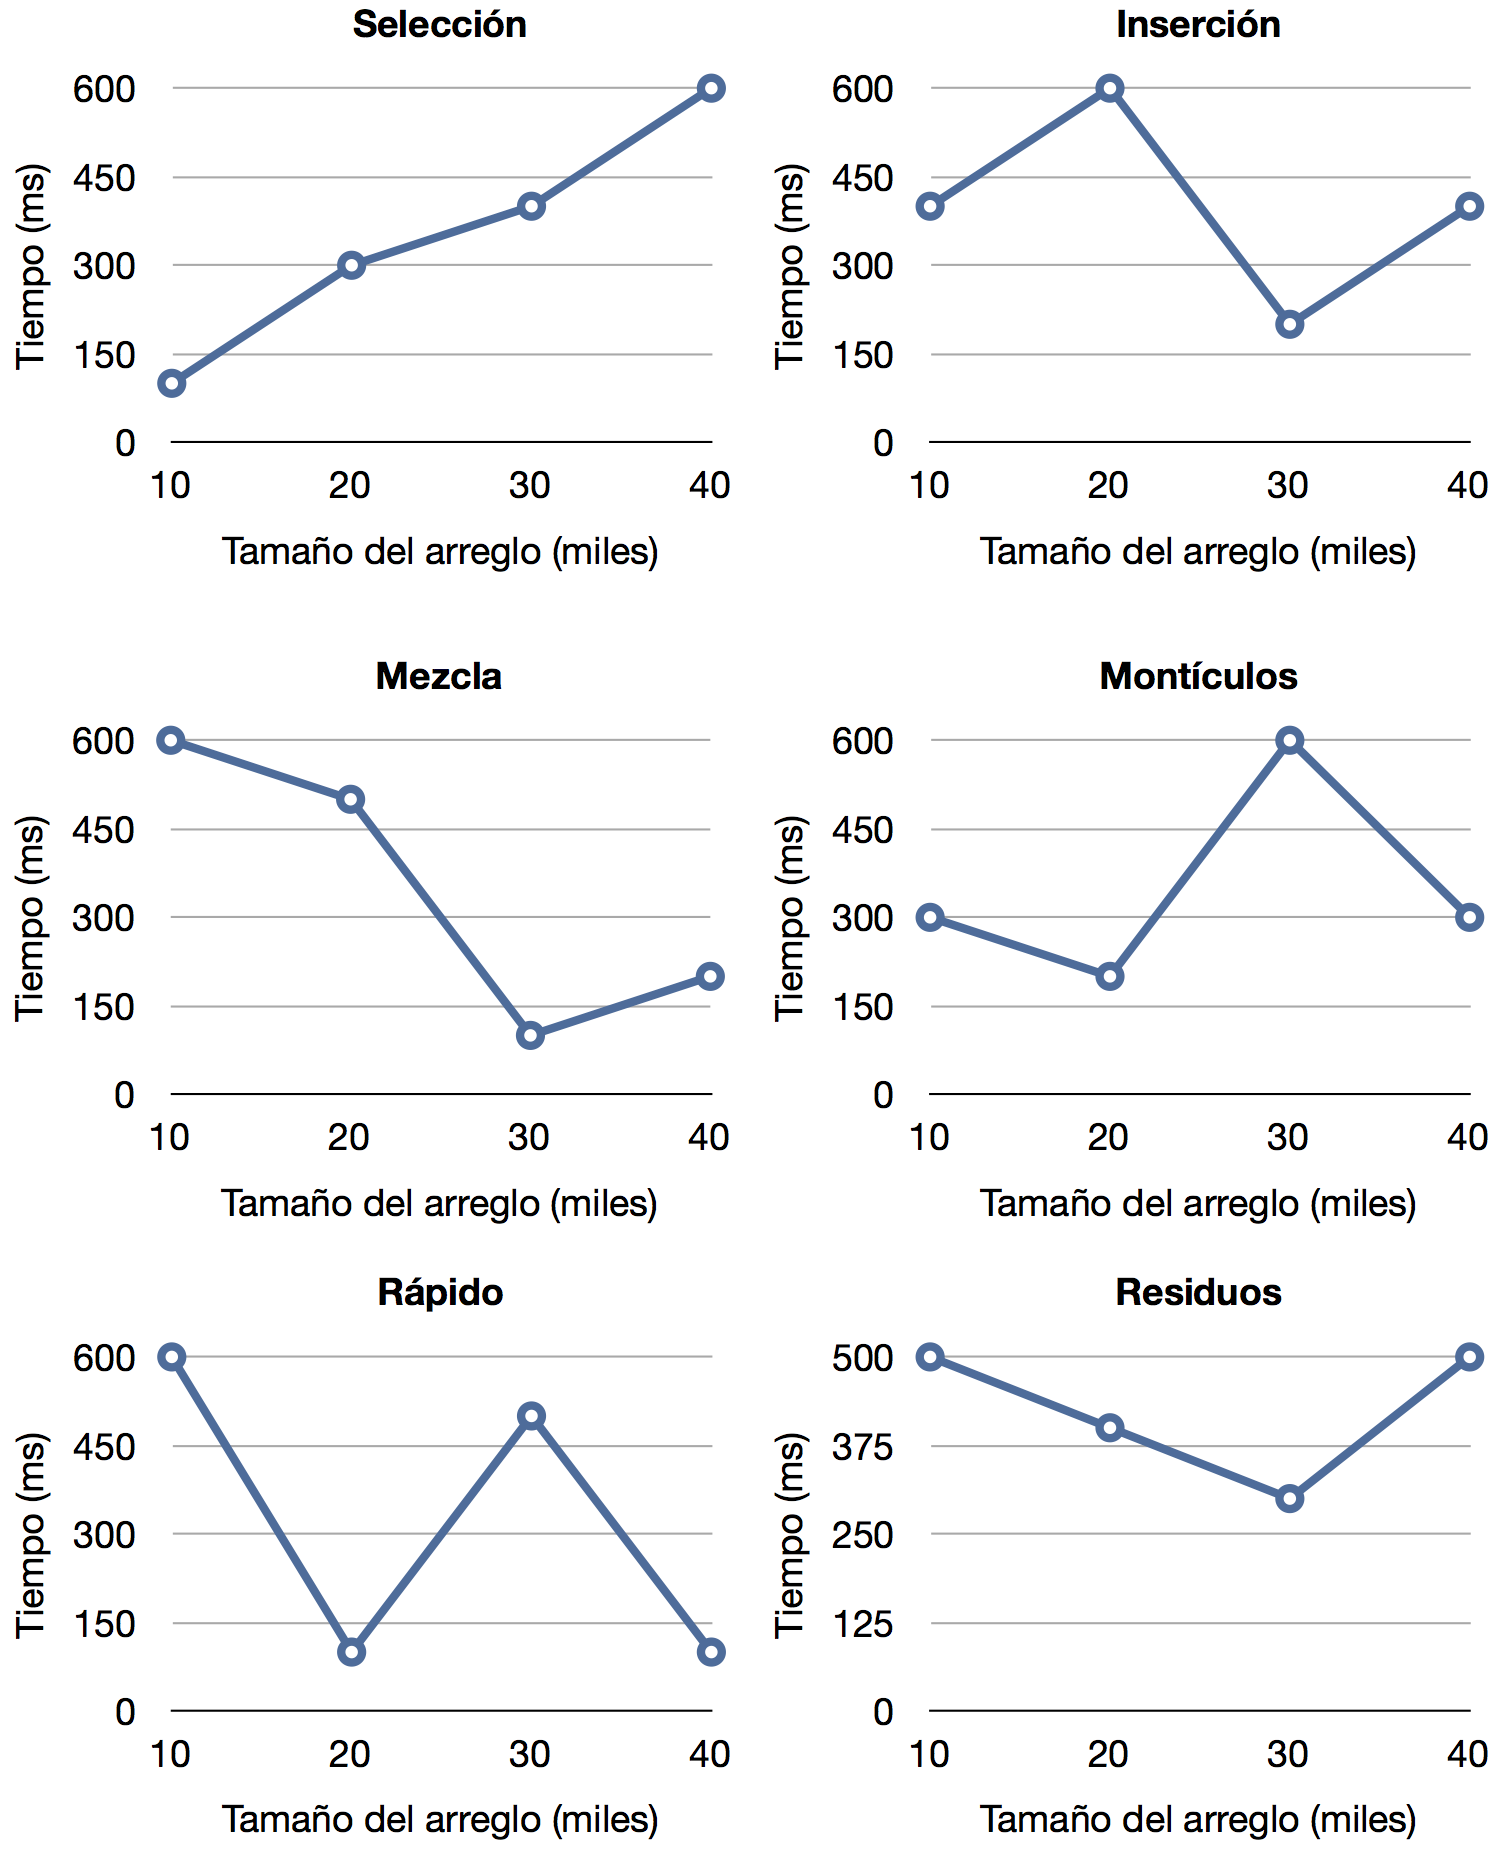
\includegraphics[scale=0.65]{lin}
\par\end{centering}

\caption{Tiempos promedio de ejecución de los algoritmos de ordenamiento por
selección, inserción, mezcla, montículos, rápido y residuos.\label{fig:lin}}
\end{figure*}

La forma de las curvas no fueron las esperadas porque inventé los números. Lorem ipsum dolor sit amet, consetetur sadipscing elitr, sed diam nonumy eirmod tempor invidunt ut labore et dolore magna aliquyam erat, sed diam voluptua. At vero eos et accusam et justo duo dolores et ea rebum. Stet clita kasd gubergren, no sea takimata sanctus est Lorem ipsum dolor sit amet. Lorem ipsum dolor sit amet, consetetur sadipscing elitr, sed diam nonumy eirmod tempor invidunt ut labore et dolore magna aliquyam erat, sed diam voluptua.

Las curvas se muestran de forma conjunta en la figura~\ref{fig:log}.


\begin{figure}[h!]
\begin{centering}
%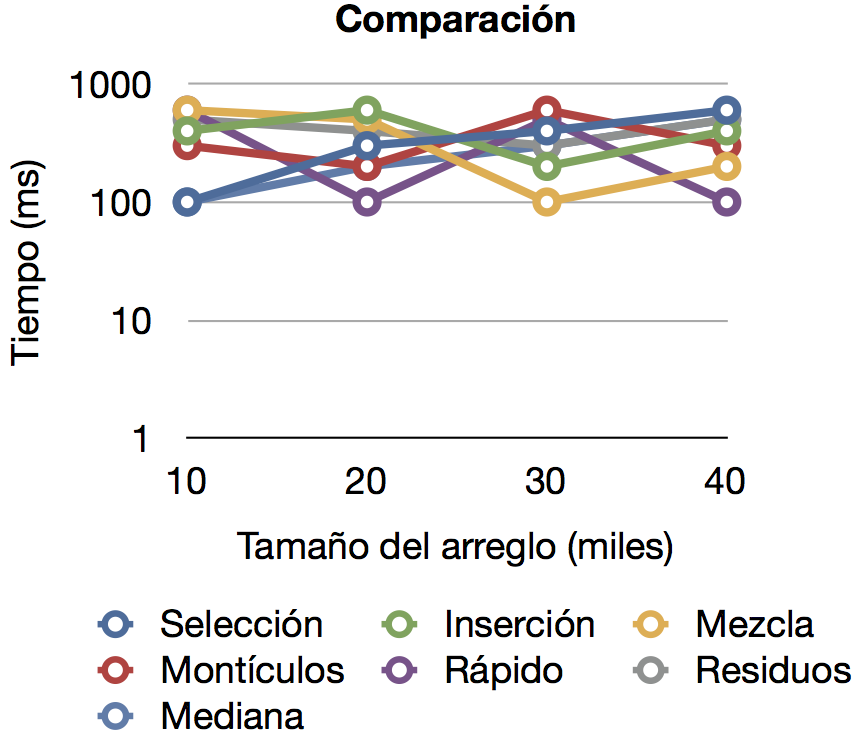
\includegraphics[width=0.62\textwidth]{log}
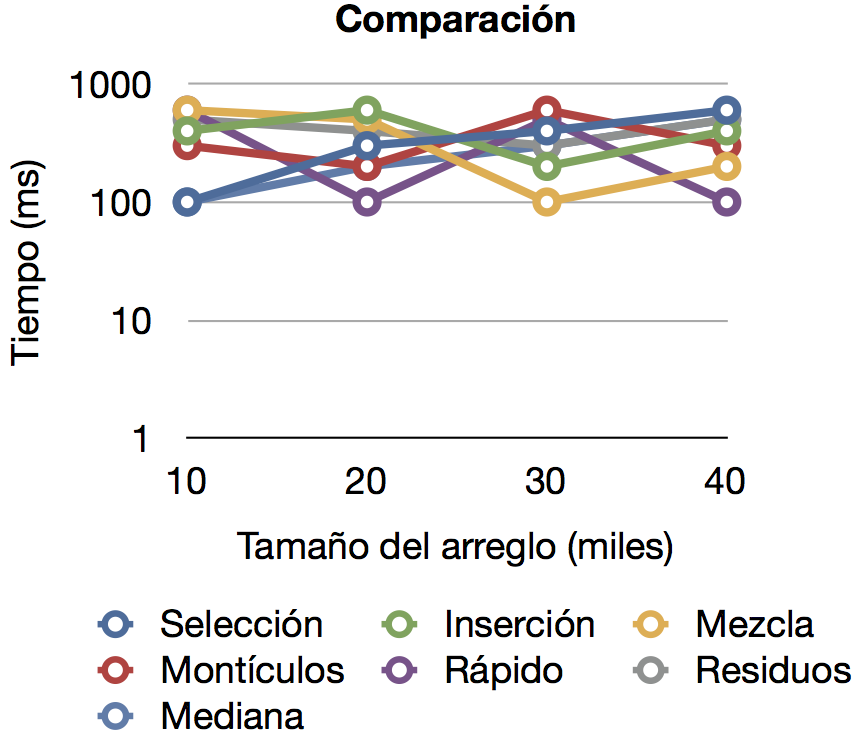
\includegraphics[scale=0.6]{log}
\par\end{centering}

\caption{Gráfico comparativo de los tiempos promedio de ejecución de algoritmos de ordenamiento.\label{fig:log}}
\end{figure}


Lorem ipsum dolor sit amet, consetetur sadipscing elitr, sed diam nonumy eirmod tempor invidunt ut labore et dolore magna aliquyam erat, sed diam voluptua. At vero eos et accusam et justo duo dolores et ea rebum. Stet clita kasd gubergren, no sea takimata sanctus est Lorem ipsum dolor sit amet. Lorem ipsum dolor sit amet, consetetur sadipscing elitr, sed diam nonumy eirmod tempor invidunt ut labore et dolore magna aliquyam erat, sed diam voluptua.

\section{Discusión}

Como primer punto, con base en los resultados presentados, se puede observar que \dots{}. Lorem ipsum dolor sit amet, consetetur sadipscing elitr, sed diam nonumy eirmod tempor invidunt ut labore et dolore magna aliquyam erat, sed diam voluptua. At vero eos et accusam et justo duo dolores et ea rebum. Stet clita kasd gubergren, no sea takimata sanctus est Lorem ipsum dolor sit amet. Lorem ipsum dolor sit amet,
consetetur sadipscing elitr, sed diam nonumy eirmod tempor invidunt.

Adicionalmente, los experimentos realizados revelan que\dots{}. Lorem ipsum dolor sit amet, consetetur sadipscing elitr, sed diam nonumy eirmod tempor invidunt ut labore et dolore magna aliquyam erat, sed diam voluptua. At vero eos et accusam et justo duo dolores et ea rebum. Stet clita kasd gubergren, no sea takimata sanctus est Lorem ipsum dolor sit amet. Lorem ipsum dolor sit amet,
consetetur sadipscing elitr, sed diam nonumy eirmod tempor invidunt.

Por otra parte, con los datos recolectados en la tabla \dots{}. Lorem ipsum dolor sit amet, consetetur sadipscing elitr, sed diam nonumy eirmod tempor invidunt ut labore et dolore magna aliquyam erat, sed diam voluptua. At vero eos et accusam et justo duo dolores et ea rebum. Stet clita kasd gubergren, no sea takimata sanctus est Lorem ipsum dolor sit amet. Lorem ipsum dolor sit amet,
consetetur sadipscing elitr, sed diam nonumy eirmod tempor invidunt.

\section{Conclusiones}

Retomando los objetivos de este trabajo, se puede concluir que\ldots{} Lorem ipsum dolor sit amet, consetetur sadipscing elitr, sed diam nonumy eirmod tempor invidunt ut labore et dolore magna aliquyam erat, sed diam voluptua. At vero eos et accusam et justo duo dolores et ea rebum. Stet clita kasd gubergren, no sea takimata sanctus est Lorem ipsum dolor sit amet. Lorem ipsum dolor sit amet, consetetur sadipscing elitr, sed diam nonumy eirmod tempor invidunt ut labore et dolore magna aliquyam erat, sed diam voluptua.




\bibliographystyle{IEEEtran}

\bibliography{Referencias}


\begin{IEEEbiography}[{

\includegraphics[width=1in, height=1.25in]{imgs/user.png}
}]%% gender neutral user by Miguel Rocha from Noun Project (CC BY 3.0)
{Your Name}
Some words about you, e.g. as a student, as a person in general, and what your interests are.

\end{IEEEbiography}




\newpage
\appendices{}


\section{Código de los algoritmos}

Esta sección no debe ir en en reporte escrito. Los siguientes bloques son solo demostrativos en caso de que considere necesario incluir código fuente o pseudocódigo en su reporte para guiar o complementar la discusión del reporte. Al igual que una figura o tabla, si agrega código fuente al reporte, debe referirse a este en el texto del documento.

El código se muestra en los algoritmos \ref{alg:saludo-tico} y \ref{alg:hello-world}. El primero es un ejemplo de código que se puede colocar en una columna. Si el código no cabe en una columna, en \protect\LaTeX{} use la versión «con estrella» del entorno «algoritmo»: \texttt{\textbackslash{}begin\{algorithm{*}\}} que se muestra en el segundo ejemplo, el cual además extrae de un archivo el contenido a mostrar.



\begin{algorithm}[h!]
\caption{Algoritmo que despliega en la salida estándar una cadena de texto.
\label{alg:saludo-tico}}

\begin{lstlisting}
int main() {
	cout << 'Pura vida!\n';
	return 0;
}
\end{lstlisting}
\end{algorithm}


\begin{algorithm*}
\caption{Primer código que normalmente se utiliza en un ejercicio de programación.
\label{alg:hello-world}}

\lstinputlisting[language={C++}]{Hello_world.cpp}
\end{algorithm*}


\end{document}

